\documentclass [11pt]{article}

\usepackage{amsmath}
\usepackage{amsfonts}
\usepackage{amssymb}
\usepackage{graphicx}
\usepackage{subcaption}
\usepackage{float}
\usepackage{fancyvrb}



\title{FYS-STK4155 Mandatory Assignment 1: \\ Regression analysis and resampling methods}
\author{Minh Chien Nguyen (davidngcz@gmail.com)}

\begin{document}
\maketitle
\nocite{*}
\begin{abstract}
The aim of this project is to compare three traditional approaches to regression analysis: Ordinary Least Squares method, Ridge regression and Lasso regression, using both simulated data and real data. In order to perform a proper assessment of the presented techniques, we employ a statistical method called k-fold cross-validation.
\end{abstract}

\section*{Introduction}
Regression is the oldest, simple and widely used supervised machine learning algorithm for data analysis. This method is mostly used for forecasting and finding out relationship between variables. The different between regression techniques is based on the number of independent variables and the type of relationship between the independent and dependent variables. Here, we will restrict ourselves to the case of polynomial regression.\\
\\
Three traditional methods of regression are recognized: Ordinary Least Squares method, Ridge regression and Lasso regression. All of them have received much attention among practitioners, as well as in academic literature.\\
\\
This text is organized as follows. Main tools and results which allow for application to fitting functions are presented in Section \ref{sec:techniques}. We further test performance of the presented methods on a Franke's
function. Finally, the techniques are applied to real data in Section \ref{sec:realdata}. In the last part of the text, we resume the principal results and suggest potential improvements in the future.
\section{Mathematical tools}
\label{sec:techniques}
This section provides an overview of basic regression methods. Preliminary knowledge of statistic is expected. There are many excellent textbooks (see e. g. \cite{abc},\cite{TRJ} and \cite{def}) which cover these topics. Here, however, the subtle mathematical issues are not addressed and we will present the main tools and results without details, but it will suffice for immediate application to fitting functions.\\

\subsection{Linear regression}
Linear regression is the most widely used statistical technique for predictive modeling, since it is very simple and often provides an good description of how the inputs affect the output.\\
Let $(x_{1},y_{1}),\ldots,(x_{N},y_{N})$ to be observed data, where each $x_{i} = (x_{i1},x_{i2},\ldots,x_{i p})$ is a vector obtained from the $i\text{th}$ measurement. The set of variables $(x_{1},\ldots,x_{N})$ is called the independent variable or the predictor variable while the set of variable $y=(y_{1},\ldots,y_{N})$is called the dependent or the response variable. \\
The goal of the regression analysis is to extract/exploit relationship between $y_i$ and $x_i$. The linear regression model assumes that there exists $\beta=(\beta_{0},\beta_{1},\ldots,\beta_{p})^{T}$ satisfying 
\begin{equation}
y_{i}=f(x_{i})=\beta_{0} + \sum_{j=1}^{p}x_{ij}\beta_{j}.
\end{equation}
The method of least squares suggest that the coefficients $\beta$ should minimize the residual sum of squares
\begin{equation}
\hat{\beta}=\text{argmin}_{\beta} ( \sum_{i=1}^{N}(y_{i}- \beta_{0}- \sum_{j=1}^{p}x_{ij}\beta_{j})^{2}).
\label{eq:ols}
\end{equation}
The unique solution to equation \eqref{eq:ols} is given by (see \cite{def})
\begin{equation}
\hat{\beta} =\left(\hat{X}^T\hat{X}\right)^{-1}\hat{X}^T\hat{y}.
\end{equation}

\subsection{Regularization}
One of the most common method to overcome overfitting is regularization. The main concept behind this approach is simplifying the model as much as possible. In other words, we reduce the magnitude of the coefficients of inputs in our model. In the following part, we present two different types of regression techniques using regularization.

\subsubsection*{Ridge Regression}
The first techniques is called ridge regression and its coefficients are defined by 
\begin{equation}
\hat{\beta}^{\text{ridge}}=\text{argmin}_{\beta} ( \sum_{i=1}^{N}(y_{i}- \beta_{0}- \sum_{j=1}^{p}x_{ij}\beta_{j})^{2}+ \lambda \sum_{j=1}^{p} \beta_{j}^{2}).
\label{eq:ridge}
\end{equation}
In equation \eqref{eq:ridge} we added an extra term, which is known as the penalty term. $\lambda \geq 0$ is called tuning parameter. It easy to see that higher the value of $\alpha$, higher is the term 
\begin{equation*}
\sum_{i=1}^{N}(y_{i}- \beta_{0}- \sum_{j=1}^{p}x_{ij}\beta_{j})^{2}+ \lambda \sum_{j=1}^{p} \beta_{j}^{2}
\end{equation*}
therefore the magnitude of coefficients $\beta$ are reduced. Roughly speaking, we punish the cost function for high values of $\beta$. It is important to note that the parameter $\lambda$ can be learned as well, using a method called cross validation that will be discussed in section \ref{sec_kcross}.
The ridge regression solution is given by
\begin{equation}
\hat{\beta} =\left(\hat{X}^T\hat{X} + \lambda I \right)^{-1}\hat{X}^T\hat{y},
\end{equation}
where $I$ is the $p \times p$ identity matrix.
\subsubsection*{Lasso Regression}
Lasso is similar to ridge, but with a small twist. The lasso estimate is in the form
\begin{equation}
\hat{\beta}^{\text{lasso}}=\text{argmin}_{\beta} ( \sum_{i=1}^{N}(y_{i}- \beta_{0}- \sum_{j=1}^{p}x_{ij}\beta_{j})^{2}+ \lambda \sum_{j=1}^{p} |\beta_{j}|).
\label{eq:lasso}
\end{equation}
An important note to notice in equation \eqref{eq:lasso} is that the only difference from ridge regression is term $\lambda \sum_{j=1}^{p} |\beta_{j}|$. Here, the method might include fewer predictors in the model, since lasso sets the irrelevant coefficient $\beta$ to zero.
\subsection{K-folds cross-variation}
\label{sec_kcross}
K-folds cross-variation is a very useful technique for calculating the performance of prediction models. The general procedure can be described as follows:
\begin{enumerate}
\item Shuffle the dataset randomly.
\item Divide the dataset into k groups.
\item For each group:
\begin{enumerate}
\item Take the group as a test data set.
\item Take the remaining groups as a training data set.
\item Fit a model on the training set and evaluate it on the test set.
\item Calculate the evaluation score.
\end{enumerate}
\item Estimate the accuracy of the model by averaging the evaluation score derived in all the $k$ cases.
\end{enumerate}
For more information about regularization, we refer to \cite{TRJ}.

\subsection{Performance criteria}
To test the performance of our results, we list the relevant criteria that we use throughout this section. In the next part, we will denote $\tilde{\hat{y}}_i$  the predicted value of the $i-th$ sample and $y_i$ is the corresponding true value.\\
\begin{enumerate}
\item Mean squared error (MSE) - measures the average of the squares of the errors, which is defined as
\begin{equation}
MSE(\hat{y},\hat{\tilde{y}}) = \frac{1}{n}
\sum_{i=0}^{n-1}(y_i-\tilde{y}_i)^2,
\end{equation}
it is clear that the smaller the value of MSE, the better the fit.
\item Coefficient of determination $R^{2}$ - is a number that indicates the proportion of the variance in the dependent variable that is predictable from the independent variable. The $R^2$ is defined as
\begin{equation}
R^2(\hat{y}, \tilde{\hat{y}}) = 1 - \frac{\sum_{i=0}^{n - 1} (y_i - \tilde{y}_i)^2}{\sum_{i=0}^{n - 1} (y_i - \bar{y})^2},
\end{equation}
where the mean value  of $\hat{y}$ is defined as $\bar{y} =  \frac{1}{n} \sum_{i=0}^{n - 1} y_i$.
\item Bias - is the difference between the expected prediction of our model and the correct value which we want to predict. Bias is defined as
\begin{equation}
Bias^2= \sum_i (f(\boldsymbol{x}_i)-E_\mathcal{L}[\hat{g}_\mathcal{L}(\boldsymbol{x}_i)])^2,
\end{equation}
where $E_{\mathcal{L}}$ denotes the expected value of the functional over the dataset $\mathcal{L}=\{\mathcal{L}_1,
\mathcal{L}_2, \ldots \}$.
\item Variance - is an error from sensitivity to small fluctuation in the training set.
\begin{equation}
Var=\sum_i E[( \hat{g}(\boldsymbol{x}_i)-E[\hat{g}(\boldsymbol{x}_i)])^2],
\end{equation}
Models with high variance usually perform very well on training data but have high error on test data.
\end{enumerate}
\section{Testing on simulated and real data}
After the theoretical considerations of the previous sections, we now want to test the performance of the presented techniques. First, we study how to fit polynomials to a Franke's function. Then we apply the methods on the polynomial approximation of digital terrain data.
\subsection{Franke's function}
\label{sebsec:franke}
In this section we perform a regression analysis of a specific two-dimensional function called Franke's
function which is defined for $x,y\in [0,1]$ as

\begin{align}
f(x,y) &= \frac{3}{4}\exp{\left(-\frac{(9x-2)^2}{4} - \frac{(9y-2)^2}{4}\right)}+\frac{3}{4}\exp{\left(-\frac{(9x+1)^2}{49}- \frac{(9y+1)}{10}\right)} \\
&+\frac{1}{2}\exp{\left(-\frac{(9x-7)^2}{4} - \frac{(9y-3)^2}{4}\right)} -\frac{1}{5}\exp{\left(-(9x-4)^2 - (9y-7)^2\right) }.
\label{eq:franke}
\end{align}

Figure \ref{fig:Franke} shows a three-dimensional plot of the Franke's function with an added stochastic noise to it using  the normal distribution $N(0,1)$. From equation \eqref{eq:franke} we know that the Franke's function is a weighted sum of four exponentials and it is clearly an infinitely differentiable function on $[0,1] \times [0,1]$. Therefore, to perform an regression analysis of this function, we will test
polynomial fits in $x$ and $y$ up to fifth order.
\begin{figure}[H]
\centering
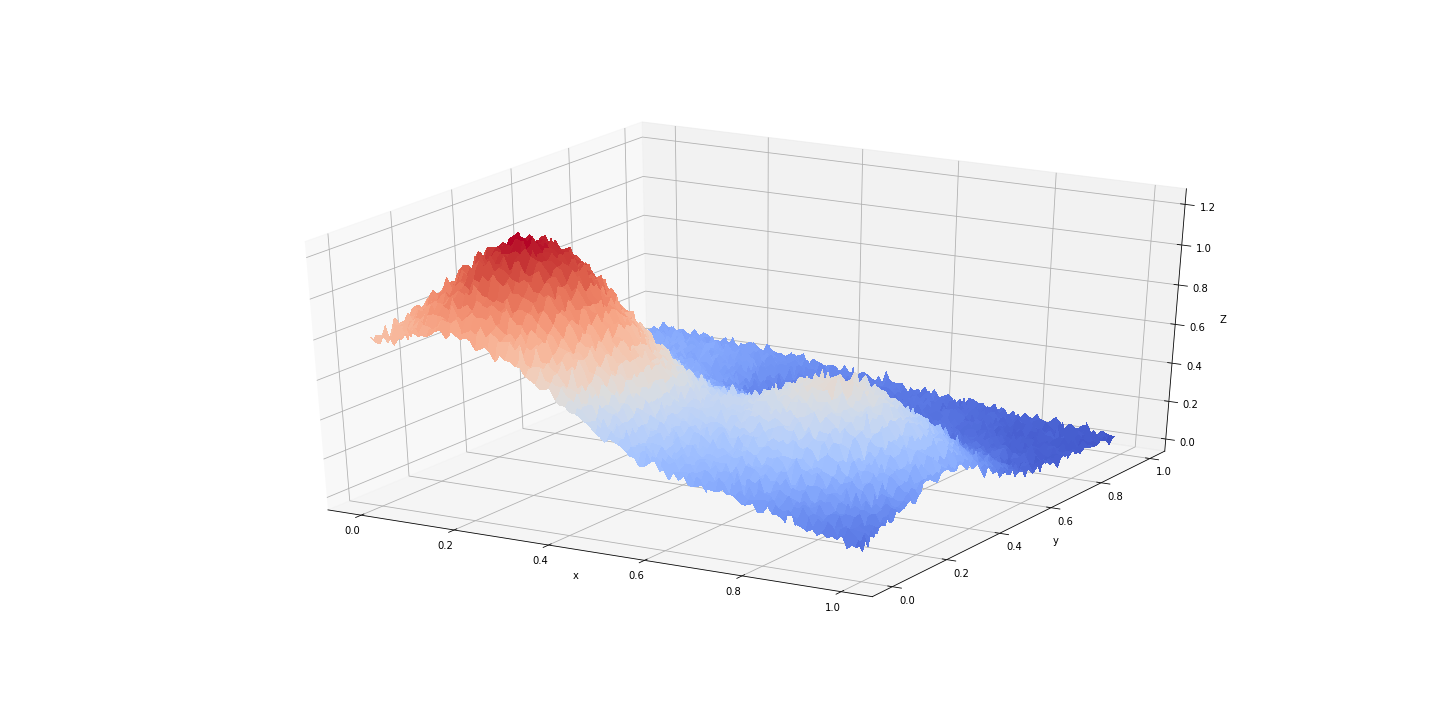
\includegraphics[width=1\textwidth]{figures/Franke.png}
        \caption{Average fitness of the best fit individual in each generation for $24$ cities using Baldwinian GA}
        \label{fig:Franke}
\end{figure}

\subsubsection{OLS}
In this part we perform an OLS regression analysis of the Franke's function. First, we generate the arrays of values for $x$ and $y$ with a step size $h=0.01$. Then, we evaluate the Franke's function adding stochastic noise $N(0,1)$. Next, we split our data set into a training set and a test set, where the training set contains $70\%$ of the original data set. Finally, we fit a OLS polynomial regression model order $3$ on the training set and evaluate it on the test set. \\
The estimation of coefficients $\beta$ and their confident intervals are shown in Table \ref{tab:olsfrane1}. The value of MSE is $0.0080$, meaning that the estimators of our model predicts observations with relatively high accuracy. The value of the coefficient of determination $R^{2}$ is $0.9015$ saying that the regression predictions approximate the real data points very well.
\begin{table}[H]
\centering
\begin{tabular}{ll}
\hline
$\beta$ & Confident interval \\ \hline
0.959   & (0.958, 0.961)     \\
-0.380  & (-0.387 ,-0.373)   \\
1.441   & (1.434, 1.448)     \\
-1.807  & (-1.820,  -1.794)  \\
-6.742  & (-6.755, -6.729)   \\
1.865   & (1.855, 1.876)     \\
1.121   & (1.113, 1.129)     \\
4.737   & (4.729, 4.745)     \\
0.461   & (0.453, 0.468)     \\
-1.445  & (-1.452, -1.437)   \\ \hline
\end{tabular}
\caption{My caption}
\label{tab:olsfrane1}
\end{table}
Now, we perform a resampling of the data for the OLS regression analysis least square regression analysis using polynomials in $x$ and $y$ up to fifth order. The process is set up as follows
\begin{enumerate}
\item Generate the arrays of values for $x$ and $y$ with a step size $h=0.01$. 
\item Evaluate the Franke's function with an added stochastic noise to it using  the normal distribution $N(0,1)$.
\item Perform resampling of the data using k-fold Cross-Validation
\item Fit the OLS regression model for each fold and each order of polynomials.
\end{enumerate}
Table \ref{tab:olsFranke} shows the results obtained using classical OLS method with resampling. We see that as the order of the polynomial fit increases the value of  the mean squared error (MSE) decreases, this means that using higher order polynomials is much more accurate. 

\begin{table}[H]
\centering
%\resizebox{\textwidth}{!}{%
\begin{tabular}{lll}
\hline
  & MSE    & R2 score \\ \hline
3 & 0.0082 & 0.9      \\
4 & 0.0044 & 0.94     \\
5 & 0.0025 & 0.97     \\ \hline
\end{tabular}%
%}
\caption{My caption}
\label{tab:olsFranke}
\end{table}
Similarly, there is an increase in the value R-square as the order of polynomial increases. In the case of polynomial fit order $5$, $R^{2}$ is $0.97$, meaning, $97\%$ of variance in $z$ is explained by the predictors. 
\begin{figure}[H]
\centering
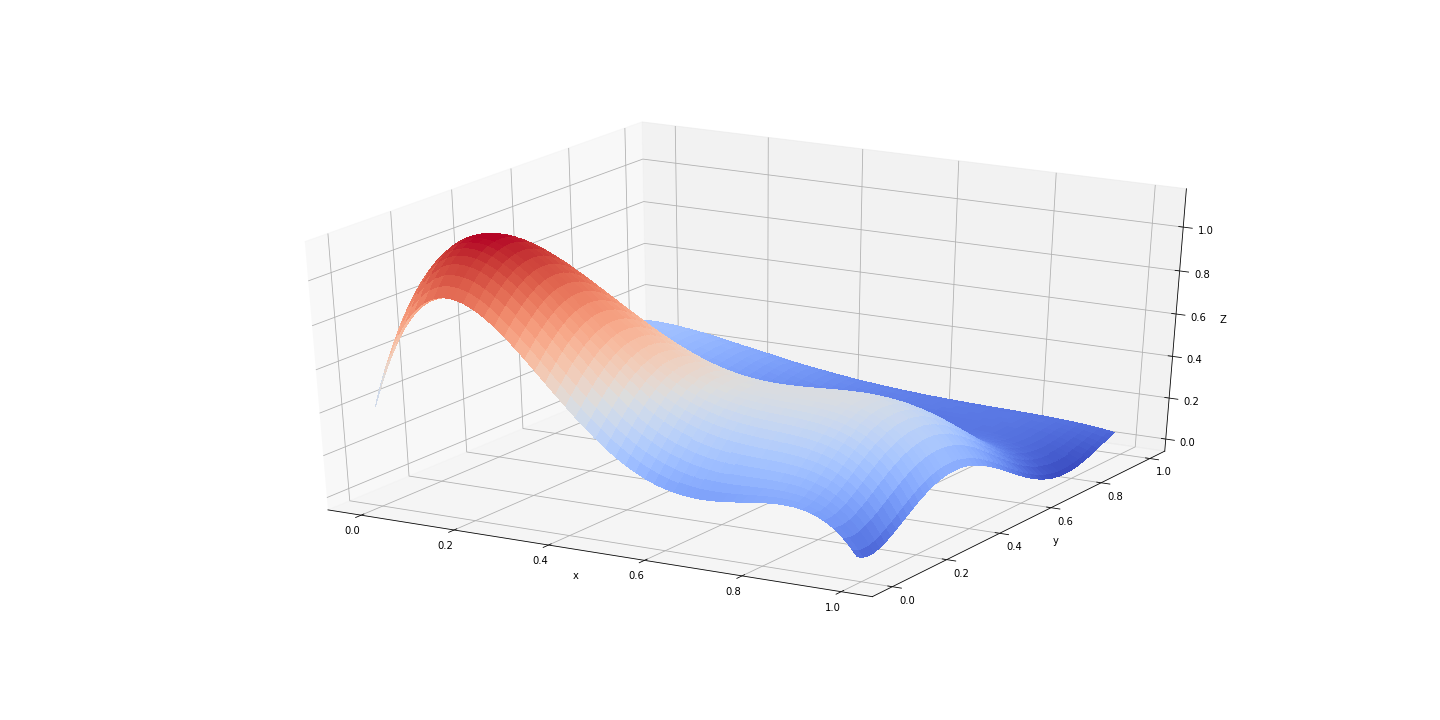
\includegraphics[width=1\textwidth]{figures/olsFranke.png}
        \caption{Average fitness of the best fit individual in each generation for $24$ cities using Baldwinian GA}
        \label{fig:olsFranke}
\end{figure}
Whenever we discuss model prediction, it is important to understand prediction errors (bias and variance). Bias for the final model is: $0.00245$ and Variance is: $5.48e-07$. We conclude that our model is underfit neither overfit, since the error of our model is relatively low.


\subsubsection{Rigde regression on the Franke function  with resampling}
In this part, we perform the same analysis as in the previous section for the Ridge regression with different values of $\lambda$ but now only with resampling.\\
As mentioned above our model is not overfit, therefore it is not surprising that the best result is obtained using low value of the tuning parameter $\lambda$. In Tables \ref{tab:ridge3}, \ref{tab:ridge4} and \ref{tab:ridge5} we see that as the value of $\lambda$ decreases the value of MSE for the Ridge regression model with resampling decreases, meanwhile the coefficient of determination $R^{2}$ is increasing.
\begin{table}[H]
\centering
\begin{tabular}{lll}
\hline
$\lambda$ & MSE    & $R^{2}$ score \\ \hline
0.001     & 0.0082 & 0.90          \\
0.01      & 0.0082 & 0.90          \\
0.1       & 0.0082 & 0.90          \\
1         & 0.0102 & 0.87          \\
10        & 0.0161 & 0.80          \\
100       & 0.0235 & 0.71          \\ \hline
\end{tabular}
\caption{order3}
\label{tab:ridge3}
\end{table}

\begin{table}[H]
\centering
\begin{tabular}{lll}
\hline
$\lambda$ & MSE    & $R^{2}$ score \\ \hline
0.001     & 0.0043 & 0.94          \\
0.01      & 0.0047 & 0.94          \\
0.1       & 0.0071 & 0.91          \\
1         & 0.0091 & 0.88          \\
10        & 0.0137 & 0.83          \\
100       & 0.0223 & 0.73          \\ \hline
\end{tabular}
\caption{order 4}
\label{tab:ridge4}
\end{table}

\begin{table}[H]
\centering
\begin{tabular}{lll}
\hline
$\lambda$ & MSE    & $R^{2}$ score \\ \hline
0.001     & 0.0027 & 0.96          \\
0.01      & 0.0037 & 0.95          \\
0.1       & 0.0056 & 0.93          \\
1         & 0.0089 & 0.89          \\
10        & 0.0124 & 0.85          \\
100       & 0.0213 & 0.74          \\ \hline
\end{tabular}
\caption{order 5}
\label{tab:ridge5}
\end{table}

\begin{figure}[H]
\centering
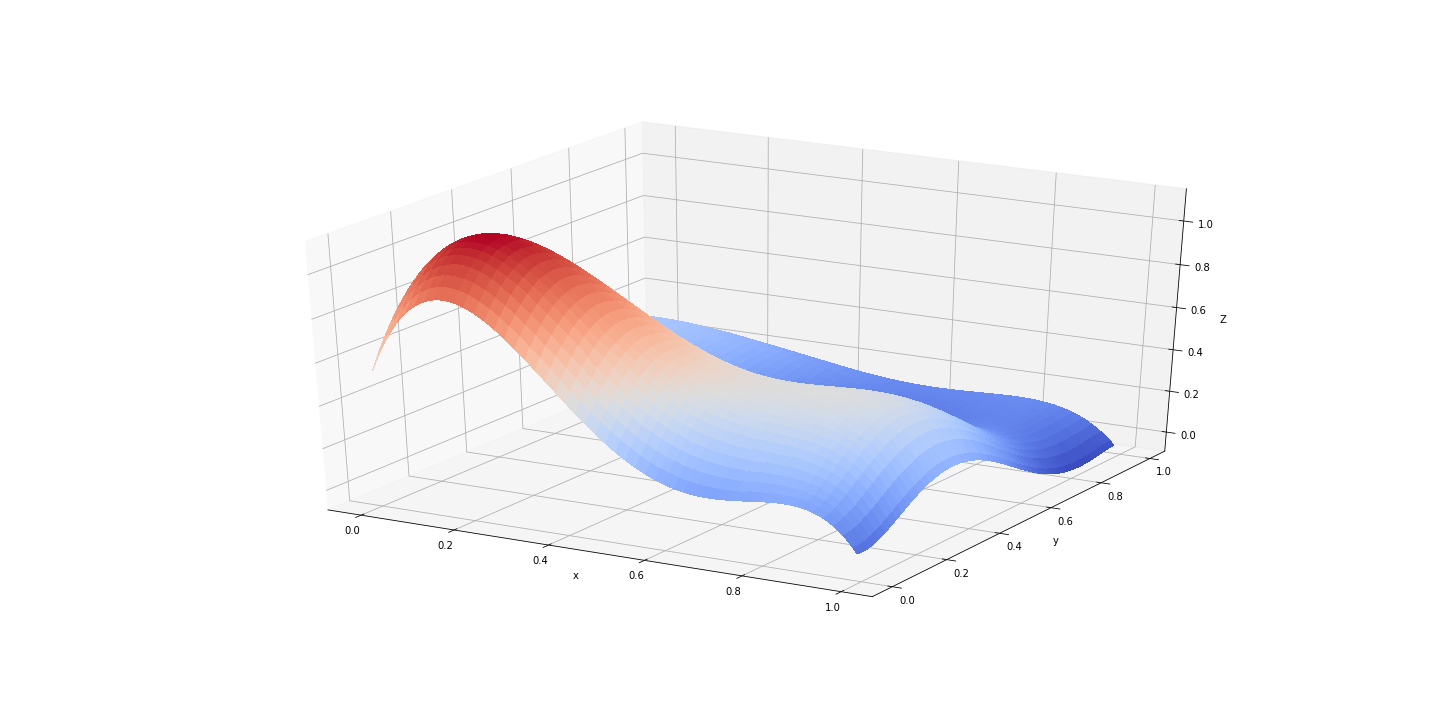
\includegraphics[width=1\textwidth]{figures/RidgeFranke.png}
        \caption{Average fitness of the best fit individual in each generation for $24$ cities using Baldwinian GA}
        \label{fig:RidgeFranke}
\end{figure}
Again, in this case the obtained results of the model using polynomial order $5$ is similar to the results using ordinary OLS model. Bias for the final Rigde model is: $0.00436$ and Variance: $8.61e-07$


\subsubsection{Lasso regression on the Franke function  with resampling}
 
This part is essentially a repeat of the previous two ones, but now with Lasso regression with resampling. Tables \ref{tab:LassoFranke3}, \ref{tab:LassoFranke4} and \ref{tab:LassoFranke5} illustrate the results for Ridge regression using different values of $\alpha$ and orders of polynomials. It is worth mentioning that for some values of $\alpha$ the coefficient of determination $R^{2}$ is negative. The reason is that by increasing $\lambda$ we reduce the magnitude of the coefficients. The higher the values of alpha is , the bigger is the penalty and therefore the magnitude of coefficients are reduced more. However, we also know that our OLS model is not overfit, which means that all predictors in our model are important and by reducing the magnitude of their coefficients we get worse predictions. 


\begin{table}[H]
\centering
\begin{tabular}{lll}
\hline
$\lambda$ & MSE    & $R^{2}$ score \\ \hline
0.001     & 0.0180 & 0.78          \\
0.01      & 0.0254 & 0.69          \\
0.1       & 0.0830 & -0.0011       \\
1         & 0.0830 & -0.0011       \\
10        & 0.0830 & -0.0011       \\
100       & 0.0830 & -0.0011       \\ \hline
\end{tabular}
\caption{3}
\label{tab:LassoFranke3}
\end{table}

\begin{table}[]
\centering
\begin{tabular}{lll}
\hline
$\lambda$ & MSE    & $R^{2}$ score \\ \hline
0.001     & 0.0142 & 0.82          \\
0.01      & 0.0254 & 0.69          \\
0.1       & 0.0830 & -0.0011       \\
1         & 0.0830 & -0.0011       \\
10        & 0.0830 & -0.0011       \\
100       & 0.0830 & -0.0011       \\ \hline
\end{tabular}
\caption{4}
\label{tab:LassoFranke4}
\end{table}

\begin{table}[]
\centering
\begin{tabular}{lll}
\hline
$\lambda$ & MSE    & $R^{2}$ score \\ \hline
0.001     & 0.0135 & 0.83          \\
0.01      & 0.0254 & 0.69          \\
0.1       & 0.0830 & -0.0011       \\
1         & 0.0830 & -0.0011       \\
10        & 0.0830 & -0.0011       \\
100       & 0.0830 & -0.0011       \\ \hline
\end{tabular}
\caption{5}
\label{tab:LassoFranke5}
\end{table}

\begin{figure}[H]
\centering
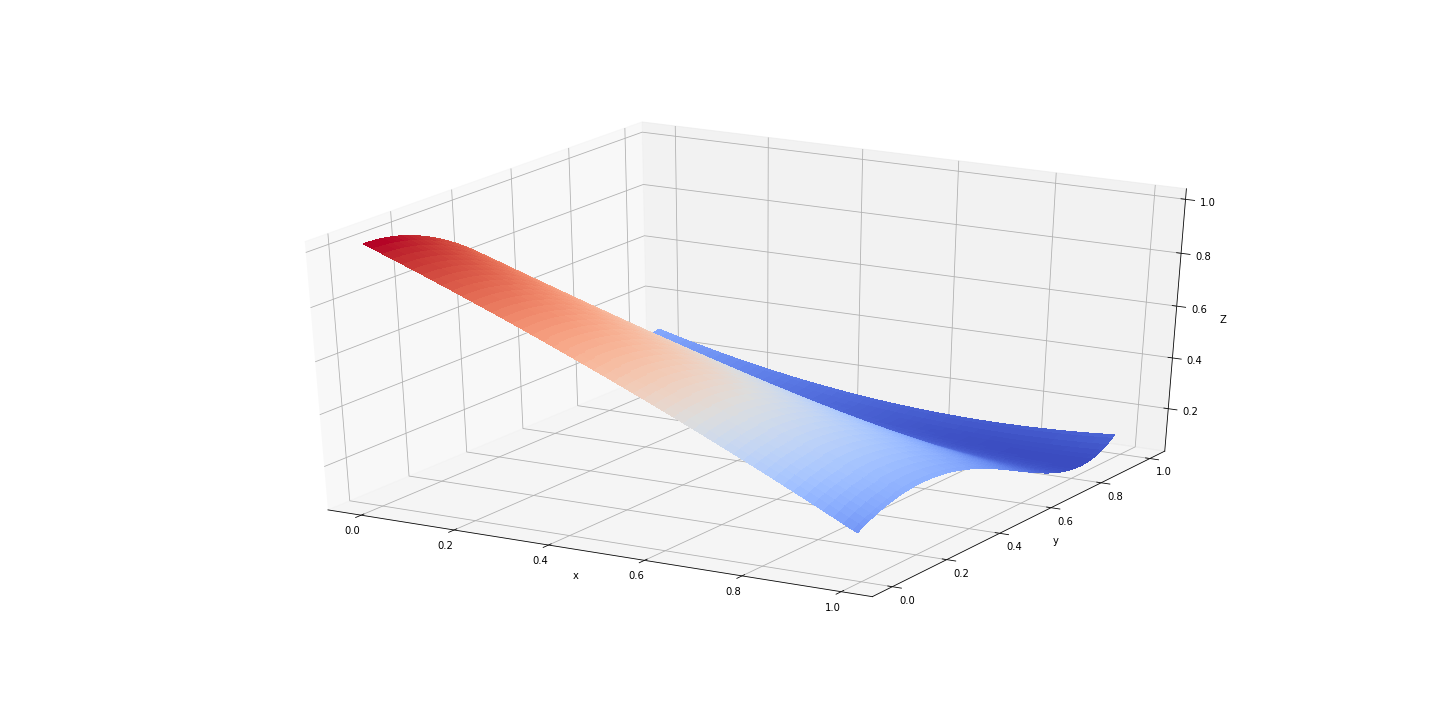
\includegraphics[width=1\textwidth]{figures/LassoFranke.png}
        \caption{Average fitness of the best fit individual in each generation for $24$ cities using Baldwinian GA}
        \label{fig:LassoFranke}
\end{figure}

Bias for the best Lasso model is $0.01349$ and Variance is $7.373e-07$. We can see that, the value for the bias of the Lasso model has been increased in comparison with the OLS and Ridge model. Therefore, in this case Lasso model is predicting worse than both OLS and Ridge.

\subsection{Real data}
\label{sec:realdata}
To illustrate the techniques described in Section \ref{sec:techniques}, we apply them to the digital terrain data from the website: https://earthexplorer.usgs.gov/.
\subsubsection{OLS real data}

\begin{table}[H]
\centering
%\resizebox{\textwidth}{!}{%
\begin{tabular}{lll}
\hline
  & MSE    & R2 score \\ \hline
3 & 305.03 & 0.71      \\
4 & 219.98 & 0.78     \\
5 & 170.80 & 0.82     \\ \hline
\end{tabular}%
%}
\caption{My caption}
\label{tab:olsTerrain}
\end{table}
Avarage Bias for the final model is: $169.51$ and avarage Variance is: $0.111$.
\subsubsection{Ridge real data}
\begin{table}[H]
\centering
\begin{tabular}{lll}
\hline
$\lambda$ & MSE    & $R^{2}$ score \\ \hline
0.001     & 304.89 & 0.71          \\
0.01      & 304.89 & 0.71          \\
0.1       & 304.89 & 0.71         \\
1         & 305.09 & 0.71         \\
10        & 321.40 & 0.66          \\
100       & 760.59 & -0.53          \\ \hline
\end{tabular}
\caption{order3}
\label{tab:ridge3Terrain}
\end{table}

\begin{table}[H]
\centering
\begin{tabular}{lll}
\hline
$\lambda$ & MSE    & $R^{2}$ score \\ \hline
0.001     & 219.86 & 0.78          \\
0.01      & 219.86 & 0.78          \\
0.1       & 219.86 & 0.78         \\
1         & 220.27 & 0.78          \\
10        & 248.02 & 0.69          \\
100       & 599.39 & -0.31          \\ \hline
\end{tabular}
\caption{order4}
\label{tab:ridge4Terrain}
\end{table}

\begin{table}[H]
\centering
\begin{tabular}{lll}
\hline
$\lambda$ & MSE    & $R^{2}$ score \\ \hline
0.001     & 170.65 & 0.82          \\
0.01      & 170.65 & 0.82          \\
0.1       & 170.65 & 0.82         \\
1         & 171.38 & 0.81          \\
10        & 209.01 & 0.70          \\
100       & 443.66 & 0.01          \\ \hline
\end{tabular}
\caption{order5}
\label{tab:ridge5Terrain}
\end{table}
Average bias for the best Rigde model is: $169.51$ and average Variance: $0.102$
\subsubsection{Lasso real data}

\section*{Conclusion}

\begin{thebibliography}{111}
\raggedright
\bibitem{abc} Christopher M. Bishop, Pattern Recognition and Machine Learning, Springer.
\bibitem{def} MARSLAND, Stephen. Machine learning: an algorithmic perspective. Chapman and Hall/CRC.
\bibitem{TRJ} Trevor Hastie, Robert Tibshirani, Jerome H. Friedman, The Elements of Statistical Learning. Springer
\end{thebibliography}
\end{document}